\documentclass{article}

%Packages
\usepackage{graphicx}
\usepackage{grffile}
\usepackage{float}

%Margins
\usepackage[
margin=2cm,
includefoot
]{geometry}

%Images
\usepackage{graphicx}

\graphicspath{{images/}}

%Headers and Footers
\usepackage{fancyhdr}
\pagestyle{fancy}
\fancyhead{}
\fancyfoot{}
\fancyfoot[R]{\thepage}
\renewcommand{\headrulewidth}{0pt}
\renewcommand{\footrulewidth}{0pt}


% Title Page
\title{Functional Specification}
\author
{  
	\\\\\\
	Stuart Andrews, 12153983 
	\\\\
	NAME, XXXXXXXX
	\\\\
	NAME, XXXXXXXX 
	\\\\
	NAME, XXXXXXXX 
	\\\\\\\\\\\\\\
}

\begin{document}
\maketitle
\thispagestyle{empty}
\newpage
\tableofcontents
\newpage

\section{Introduction}
\section{Vision}
\section{Background}
\section{Functional Requirements and Application Design}
\subsection{Use case prioritization}
\subsubsection{Application Server}
\begin{enumerate}
	\item	MQTT Server Startup - Critical
	\item	Firebase Authorisation - Critical
	\item	Validate ID - Important
	\item	Storing Data in Firebase - Critical
\end{enumerate}
\subsubsection{Firmware}
\begin{enumerate}
	\item	Particle Photon Connecting to Server - Critical
\end{enumerate}
\subsubsection{Web}
\begin{enumerate}
	\item	User Add Device - Critical
	\item	Create Firebase Database - Critical
	\item	User Registration - Important
	\item	User Login - Important
	\item	Retrieve Data  - Important
\end{enumerate}
\subsection{Use case/Services contracts}
\subsubsection{Application Server}
\begin{enumerate}
	\item	MQTT Server Startup
	\begin{enumerate}
		\item  Pre-Conditions
		\begin{enumerate}
			\item  	Server.conf configuration file needs to be present in order for the Server to start listening for incoming MQTT Connection and 
			Publish requests on the correct ports.
			\item	Server throws a MissingConfigFileException if the Server.conf file is not present.
		\end{enumerate}
		\item  Post-Conditions		
		\begin{enumerate}
			\item	Server can receive MQTT requests.
		\end{enumerate}
	\end{enumerate}
		\end{enumerate}
	\subsubsection{Firebase}
	\begin{enumerate}
		\item	Firebase Authorisation
	\begin{enumerate}
		\item  Pre-Conditions
		\begin{enumerate}
			\item	auth.json file needs to be present in order to achieve authorisation for powercloud-bf968.firebaseio.com.
			\item	Device must have authorisation to access Firebase.
			\item	Server throws a MissingAuthorisationFileException.
		\end{enumerate}
		\item  Post-Conditions		
		\begin{enumerate}
			\item	Device can save and retrieve data to and from Firebase.
		\end{enumerate}
	\end{enumerate}
	\item Validate ID
	\begin{enumerate}
		\item  Pre-Conditions
		\begin{enumerate}
			\item	The Particle Photon must have connected to the server.
			\item	Device ID must be in Firebase, else it will throw a DeviceNotFoundException.
		\end{enumerate}
		\item  Post-Conditions		
		\begin{enumerate}
			\item	The ValidateID function calls the store function, and attempts to store the data.
		\end{enumerate}
	\end{enumerate}
	\item	Storing Data in Firebase
	\begin{enumerate}
		\item  Pre-Conditions
		\begin{enumerate}
			\item	The Device ID must be valid, before an attempt to store can be made.
			\item	The storeData object must be valid.
			\item	Upon failure a StoreException must be thrown.
		\end{enumerate}
		\item  Post-Conditions		
		\begin{enumerate}
			\item	The data is stored in Firebase under the correct branch.
		\end{enumerate}
	\end{enumerate}
\end{enumerate}
	\subsubsection{Firmware}
	\begin{enumerate}
	\item	Particle Photon Connecting to Server	
	\begin{enumerate}
		\item  Pre-Conditions
		\begin{enumerate}
			\item	The Photon must have the correct addresses, i.e. port number and ip/domain name.
		\end{enumerate}
		\item  Post-Conditions		
		\begin{enumerate}
			\item	The Photon can then begin transmitting data.
		\end{enumerate}
	\end{enumerate}
\end{enumerate}
	\subsubsection{Web}
		\begin{enumerate}
	\item	Create Firebase Database
	\begin{enumerate}
		\item  Pre-Conditions
		\begin{enumerate}
			\item	Client must have a gmail account.
			\item	Client must create their own Firebase account. i.e. powercloud-bf968.
		\end{enumerate}
		\item  Post-Conditions		
		\begin{enumerate}
			\item	Client can visit firebase.google.com and view their Firebase Data
		\end{enumerate}
	\end{enumerate}
	\item	User Registration
	\begin{enumerate}
		\item  Pre-Conditions
		\begin{enumerate}
			\item	Client must register with:
			\begin{enumerate}
				\item	namecompany name.
				\item	email address.
				\item	password.
				\item	name of Firebase account i.e. powercloud-bf968.
			\end{enumerate}
		\end{enumerate}
		\item  Post-Conditions		
		\begin{enumerate}
			\item	Firebase creates a user entry.
		\end{enumerate}
	\end{enumerate}
	\item	User Login
	\begin{enumerate}
		\item  Pre-Conditions
		\begin{enumerate}
			\item	Client must be registered.
			\item	Client must login in with an email address or username, and password.
		\end{enumerate}
		\item  Post-Conditions		
		\begin{enumerate}
			\item	Client will have access to all devices, will be able to add and remove devices, and retrieve and observe data.
		\end{enumerate}
	\end{enumerate}
	\item	User Add Device
	\begin{enumerate}
		\item  Pre-Conditions
		\begin{enumerate}
			\item	Client must be logged in.
			\item	Client must have necessary authorisation.
			\item	Client must provide the following details:
			\begin{enumerate}
				\item	Device id.
				\item	Device appliance, i.e. the appliance who's value it will be reading.
				\item	Device name.
			\end{enumerate}
		\end{enumerate}
		\item  Post-Conditions		
		\begin{enumerate}
			\item	A sequential entry, i.e. 0,1,2,3...n, will be made in the Firebase Database.
		\end{enumerate}
	\end{enumerate}
	\item	Retrieve Data
	\begin{enumerate}
		\item  Pre-Conditions
		\begin{enumerate}
			\item	Client must be logged in.
			\item	Client must have necessary authorisation.
			\item	Client must have devices listed, i.e. devices that have already been added.
		\end{enumerate}
		\item  Post-Conditions		
		\begin{enumerate}
			\item	Returns a JSON object from Firebase containing all the data concerning that specific device. Database.
		\end{enumerate}
	\end{enumerate}
\end{enumerate}
\subsection{Required functionality}
\subsection{Process specifications}
\subsubsection{Store Process}
	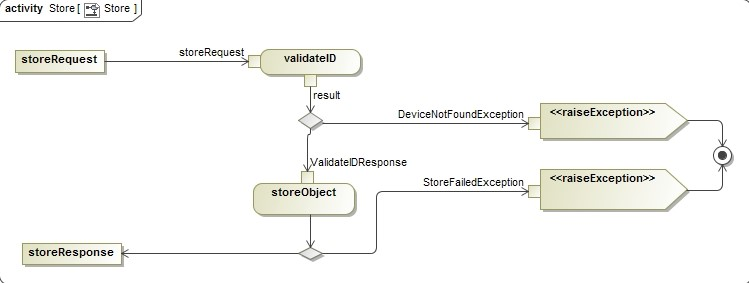
\includegraphics[width=\textwidth]{images/Store.jpg}  \\
\subsection{Domain Model}
\section{Open Issues}
\end{document}          
